% Models
\section{Models}\label{models}
	This section defines the models we use for the different network types. We define a graph
	based representation for road and transit networks. Then both graphs are combined
	into a linked graph, making it possible to have one graph for the whole network.
	Afterwards an alternative representation for transit networks is shown.
	
% Road graph
\subsection{Road graph}
	A road network typically is time independent. It consists of geographical locations and roads connecting them with each other.
	We assume that a road can be taken at any time, with no time dependent constraints.
	
	Modeling the network as graph is straightforward, \defref{roadGraph} goes into detail.
	\begin{mydef}\label{roadGraph}
		A \textnormal{road graph} is a graph $G = (V, E)$ with a set of geographic coordinates
		\begin{align*}
			V = \{(\phi, \lambda) | \phi \in \left(-\frac{\pi}{2}, \frac{\pi}{2}\right), \lambda \in \left[-\pi, \pi\right)\},
		\end{align*}
		for example road junctions.
		There is an edge $(u, w, v) \in E$ iff there is a road connecting the location $u$ with the location
		$v$, which can be taken in that direction. The weight $w$ of the edge is the average time needed
		to take the road from $u$ to $v$ using a car, measured in seconds.
	\end{mydef}
	% Road graph example
	\begin{figure}[!ht]
		 \begin{center}
			\includegraphics[scale=0.5]{res/road_network}\\
			\qquad\\
			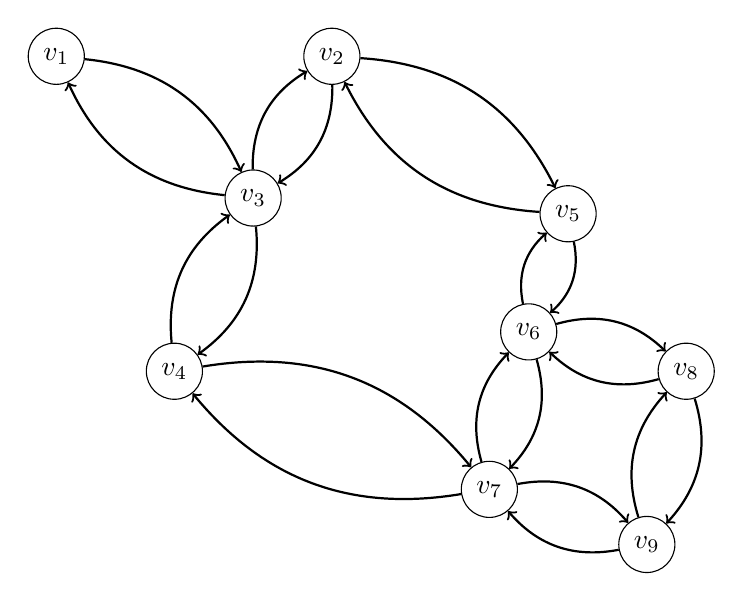
\begin{tikzpicture}[y = -1cm]
			 	% Nodes
			 	\node[circle, draw] (v1) at (0, 0) {$v_1$};
			 	\node[circle, draw] (v2) at (3.5, 0) {$v_2$};
			 	\node[circle, draw] (v3) at (2.5, 1.8) {$v_3$};
			 	\node[circle, draw] (v4) at (1.5, 4) {$v_4$};
			 	
			 	\node[circle, draw] (v5) at (6.5, 2) {$v_5$};
			 	\node[circle, draw] (v6) at (6, 3.5) {$v_6$};
			 	\node[circle, draw] (v7) at (5.5, 5.5) {$v_7$};
			 	
			 	\node[circle, draw] (v8) at (8, 4) {$v_8$};
			 	\node[circle, draw] (v9) at (7.5, 6.2) {$v_9$};
			 	
			 	% Edges
			 	\draw[thick, ->] (v1) to [bend left] (v3);
			 	\draw[thick, ->] (v3) to [bend left] (v1);
			 	
			 	\draw[thick, ->] (v3) to [bend left] (v2);
			 	\draw[thick, ->] (v2) to [bend left] (v3);
			 	\draw[thick, ->] (v3) to [bend left] (v4);
			 	\draw[thick, ->] (v4) to [bend left] (v3);
			 	
			 	\draw[thick, ->] (v2) to [bend left] (v5);
			 	\draw[thick, ->] (v5) to [bend left] (v2);
			 	\draw[thick, ->] (v4) to [bend left] (v7);
			 	\draw[thick, ->] (v7) to [bend left] (v4);
			 	
			 	\draw[thick, ->] (v5) to [bend left] (v6);
			 	\draw[thick, ->] (v6) to [bend left] (v5);
			 	\draw[thick, ->] (v6) to [bend left] (v7);
			 	\draw[thick, ->] (v7) to [bend left] (v6);
			 	
			 	\draw[thick, ->] (v6) to [bend left] (v8);
			 	\draw[thick, ->] (v8) to [bend left] (v6);
			 	\draw[thick, ->] (v7) to [bend left] (v9);
			 	\draw[thick, ->] (v9) to [bend left] (v7);
			 	
			 	\draw[thick, ->] (v8) to [bend left] (v9);
			 	\draw[thick, ->] (v9) to [bend left] (v8);
			\end{tikzpicture}
		\end{center}
		\caption{Example of a road network with its corresponding road graph. White connections indicate roads,
			dark gray rectangles represent houses or other static objects.
			Geographical coordinates for each node as well as edge weights are omitted in the graph illustration.}
		\label{roadGraphExample}
	\end{figure}\quad\\
	\figref{roadGraphExample} shows a constructed example road network with the corresponding road graph.
	Note that two way streets result in two edges, one edge for every direction the road can be taken.\\\\
	Since edge weights are represented as average time it needs to take the road, it is possible to encode different road types.
	For example the average speed on a motorway is much higher than on a residential street. As such, the weight of an edge
	representing a motorway is much smaller than the weight of an edge representing a residential street.
	
	While the example has exactly one node per road junction this must not always be the case. Typical real world data often consists
	of multiple nodes per road segment. However, \defref{roadGraph} is still valid for such data as long as there are edges
	between the nodes if and only if there is a road connecting the locations.

% Transit graph
\subsection{Transit graph}
	Transit networks can be modeled similar to road graphs. The key difference is that transit networks are time dependent
	while road networks typically are not. For example an edge connecting \textit{Freiburg main station} with \textit{Karlsruhe main station}
	can not be taken at any time since trains and other transit vehicles only depart at certain times. The schedule might even change
	at different days.\\\\
	The difficulty lies in modeling time dependence in a static graph. There are two common approaches to that problem.\\\\
	The first approach is called \textit{time-dependent}. There edge weights are not static numbers but functions that take a
	date with time and compute the cost it needs to take the edge when starting at the given time.
	This includes waiting time. As an example assume an edge $(u, c, v)$ with the cost function $c$. The edge represents a
	train connection and the travel time are $10$ minutes. However, the train departs at \timef{10}{15}{am} am but the starting time
	is \timef{10}{00}{am}. The cost function thus computes a waiting time of $15$ minutes plus the travel time of $10$ minutes.
	Resulting in an edge weight of $25$ minutes.
	
	The main problem with this model is that it makes pre-computations for route planning very difficult as
	the starting time is not known in advance.\\\\
	The second approach is called \textit{time-expanded}. There idea is to remove any time dependence
	from the graph by creating additional nodes for every event at a station. A node then also has a time information
	next to its geographic location.
	\begin{mydef}\label{simpleTransitGraph}
		A \textnormal{time expanded transit graph} is a graph $G = (V, E)$ with a set of events at geographic coordinates
		\begin{align*}
			V = \{(\phi, \lambda, t, e) | \phi \in \left(-\frac{\pi}{2}, \frac{\pi}{2}\right), \lambda \in \left[-\pi, \pi\right),
			t \text{ time}, e \in \{\text{arrival}, \text{departure}\}\},
		\end{align*}
		for example a train arriving at a train station at a certain time.
		
		A node $(\phi, \lambda, t, e) \in V$ is an \textnormal{arrival node} if $e = \text{arrival}$, analogously it is a
		\textnormal{departure node} for $e = \text{departure}$. For a node $v \in V$, $v_\phi$ and $v_\lambda$ denote its location,
		$v_t$  its time and $v_e$ its event type.
		
		It must be ensured that each connection starts with an arrival node.\\\\
		There is an edge $(u, w, v) \in E$ iff
		\begin{itemize}
			\item[1.] $u_e = \text{departure} \land v_e = \text{arrival}$ such that there is a vehicle departing
			from $u$ at time $u_t$ which arrives at $v$ at time $v_t$ without stops in between, or
			\item[2.] $u_e = \text{arrival} \land v_e = \text{departure}$
			such that $u$ and $v$ belong to the same connection. For example a train arriving at a station
			and then departing again, or
			\item[3.] $u_e = \text{arrival} \land v_e = \text{arrival}$
			such that $v$ is the node at the same coordinates than $u$ with the smallest time $v_t$ that is still
			greater than $u_t$. This edge represents exiting a vehicle and waiting for another connection. That is
			\begin{align*}
				\forall v' \in V \setminus \{v\}	&: v'_\phi = u_\phi \land v'_\lambda = u_\lambda \land v'_e = \text{arrival} \land v'_t \ge u_t\\
									&\Rightarrow v'_t - u_t > v_t - u_t.
			\end{align*}
		\end{itemize}
		The weight $w$ of an edge $(u, w, v)$ is the difference between both nodes times, that is
		\begin{align*}
			w	&= v_t - u_t.
		\end{align*}
		Note that weights are still positive since $v_t \ge u_t$ always holds due to construction.
	\end{mydef}
	% Transit graph example
	\begin{figure}[!ht]
		 \begin{center}
			\begin{tabular}{|c||c|cc|c|}
				\hline
				$\longrightarrow$	&Freiburg Hbf			&\multicolumn{2}{c|}{Offenburg}					&Karlsruhe Hbf\\
							&\small{\texttt{departure}}	&\small{\texttt{arrival}}		&\small{\texttt{departure}}	&\small{\texttt{arrival}}\\\hline
				ICE 104		&\timef{3}{56}{pm}		&\timef{4}{28}{pm}		&\timef{4}{29}{pm}		&\timef{4}{58}{pm}\\
				RE 17024		&\timef{4}{03}{pm}		&\timef{4}{50}{pm}		&					&\\
				RE 17322		&					&					&\timef{4}{35}{pm}		&\timef{5}{19}{pm}\\\hline\hline
				$\longleftarrow$	&\small{\texttt{arrival}}		&\small{\texttt{departure}}	&\small{\texttt{arrival}}		&\small{\texttt{departure}}\\\hline
				ICE  79		&\timef{8}{10}{pm}		&					&					&\timef{7}{10}{pm}\\\hline
			\end{tabular}\\\vphantom{a}\quad\\
			\begin{tikzpicture}[y = -1cm]
			 	% Nodes
			 	% Time line
			 	\node[left] at (-1, 0) {\timef{3}{56}{pm}};
			 	\node[left] at (-1, 1) {\timef{4}{03}{pm}};
			 	\node[left] at (-1, 1.5) {\timef{4}{28}{pm}};
			 	\node[left] at (-1, 2) {\timef{4}{29}{pm}};
			 	\node[left] at (-1, 3) {\timef{4}{35}{pm}};
			 	\node[left] at (-1, 4) {\timef{4}{50}{pm}};
			 	\node[left] at (-1, 4.5) {\timef{4}{58}{pm}};
			 	\node[left] at (-1, 5.5) {\timef{5}{19}{pm}};
			 	\node[left] at (-1, 6.75) {\timef{7}{10}{pm}};
			 	\node[left] at (-1, 7.5) {\timef{8}{10}{pm}};
			 	
			 	% Freiburg Hbf
			 	\node[above = 0.75cm] at (0.5, 0) {Freiburg Hbf};
			 	
			 	\node[circle, draw, preaction={fill = red!20}, pattern=north west lines, pattern color=white] (f2) at (0, 0) {\phantom{v}};
			 	\node[circle, draw, preaction={fill = blue!20}, pattern=dots, pattern color=white] (f1) at (1, 0) {\phantom{v}};
			 	
			 	\node[circle, draw, preaction={fill = red!20}, pattern=north west lines, pattern color=white] (f5) at (0, 1) {\phantom{v}};
			 	\node[circle, draw, preaction={fill = blue!20}, pattern=dots, pattern color=white] (f3) at (1, 1) {\phantom{v}};
			 	
			 	\node[circle, draw, preaction={fill = red!20}, pattern=north west lines, pattern color=white] (f4) at (0, 7.5) {\phantom{v}};
			 				 	
			 	% Offenburg
			 	\node[above = 0.75cm] at (3.5, 0) {Offenburg};
			 	
			 	\node[circle, draw, preaction={fill = red!20}, pattern=north west lines, pattern color=white] (o3) at (3, 1.5) {\phantom{v}};
			 	\node[circle, draw, preaction={fill = blue!20}, pattern=dots, pattern color=white] (o4) at (4, 2) {\phantom{v}};
			 	
			 	\node[circle, draw, preaction={fill = red!20}, pattern=north west lines, pattern color=white] (o1) at (3, 3) {\phantom{v}};
			 	\node[circle, draw, preaction={fill = blue!20}, pattern=dots, pattern color=white] (o2) at (4, 3) {\phantom{v}};
			 	
			 	\node[circle, draw, preaction={fill = red!20}, pattern=north west lines, pattern color=white] (o5) at (3, 4) {\phantom{v}};
			 	
			 	% Karlsruhe Hbf
			 	\node[above = 0.75cm] at (6.5, 0) {Karlsruhe Hbf};
			 	
			 	\node[circle, draw, preaction={fill = red!20}, pattern=north west lines, pattern color=white] (k3) at (6, 4.5) {\phantom{v}};
			 	
			 	\node[circle, draw, preaction={fill = red!20}, pattern=north west lines, pattern color=white] (k1) at (6, 5.5) {\phantom{v}};
			 	
			 	
			 	\node[circle, draw, preaction={fill = red!20}, pattern=north west lines, pattern color=white] (k4) at (6, 6.5) {\phantom{v}};
			 	\node[circle, draw, preaction={fill = blue!20}, pattern=dots, pattern color=white] (k2) at (7, 7) {\phantom{v}};
			 	
			 	% Edges
			 	% ICE 104
			 	\draw[thick, ->] (f2) to node[above] {$0$} (f1);
			 	\draw[thick, ->] (f1) to node[above right] {$32$} (o3);
			 	\draw[thick, ->] (o3) to node[above] {$1$} (o4);
			 	\draw[thick, ->] (o4) to node[above right] {$29$} (k3);
			 	
			 	% RE 17024
			 	\draw[thick, ->] (f5) to node[above] {$0$} (f3);
			 	\draw[thick, ->] (f3) to node[above right] {$47$} (o5);
			 	
			 	% RE 17322
			 	\draw[thick, ->] (o1) to node[above] {$0$} (o2);
			 	\draw[thick, ->] (o2) to node[below left] {$44$} (k1);
			 	
			 	% ICE 79
			 	\draw[thick, ->] (k4) to node[above] {$0$} (k2);
			 	\draw[thick, ->] (k2) to node[above] {$60$} (f4);
			 	
			 	% Waiting arcs
			 	\draw[color= red, thick, dashed, ->] (f2) to node[left] {$7$} (f5);
			 	\draw[color= red, thick, dashed, ->] (f5) to node[right] {$247$} (f4);
			 	
			 	\draw[color= red, thick, dashed, ->] (o3) to node[right] {$7$} (o1);
			 	\draw[color= red, thick, dashed, ->] (o1) to node[right] {$15$} (o5);
			 	
			 	\draw[color= red, thick, dashed, ->] (k3) to node[right] {$21$} (k1);
			 	\draw[color= red, thick, dashed, ->] (k1) to node[left] {$111$} (k4);
			\end{tikzpicture}
		\end{center}
		\caption{Example of a transit network with its corresponding time expanded transit graph.
			The table shows an excerpt of a train schedule. Nodes with stripes are arrival nodes,
			dotted nodes represent departure nodes. Regular edges indicate a train connection
			and dashed edges waiting arcs. Edge weights are measured in minutes.}
		\label{transitGraphExample}
	\end{figure}\quad\\
	\defref{simpleTransitGraph} defines such a time expanded transit graph and \figref{transitGraphExample} shows an example.
	For simplicity it is assumed that the trains have no stops other than shown in the schedule. The schedule lists four trains:
	\begin{itemize}
		\item[1.] The ICE 104 which travels from Freiburg Hhbf to Karlsruhe Hbf via Offenburg,
		\item[2.] the RE 17024 connecting Freiburg Hbf with Offenburg,
		\item[3.] the RE 17322 driving from Offenburg to Karlsruhe Hbf and
		\item[4.] ICE 79 which travels in the opposite direction, connecting Karlsruhe Hbf with Freiburg without intermediate stops.
	\end{itemize}
	For connections that start at a station, like the $ICE 104$ in Freiburg Hbf an additional arrival node is introduced
	in the transit graph. The arrival node has the same time than its corresponding departure node, the connecting
	edge has a weight of $0$ minutes. The additional node is necessary to fulfil the requirement of
	\defref{simpleTransitGraph} that all connections start with an arrival node. It is also necessary for correctness as it must
	be possible to transfer from an arriving train to another train that starts at station. For example to transfer from ICE 104
	to RE 17322 in Offenburg, which is represented by the waiting arc with cost $7$ minutes.\\\\
	As seen in the example the resulting graph has no time dependency anymore and is static, as well as all edge weights.
	The disadvantage is that the graph size dramatically increases as a new node is introduced for every single event.
	In order to limit the growth we assume that a schedule is the same every day and does not change. In fact, most schedules are
	stable and often change only slightly, for example on weekends or at holidays. In practice hybrid models can be used for
	those exceptions.
% Link graph
\subsection{Link graph}
	blabla

% Timetable
\subsection{Timetable}
	blabla